\section{Introduction}
Organic scintillators (such as
toluene, polystyrene, and naphthalene) containing wave-length shifting
additives in solution
have long been popular elements in detectors used
in particle physics, nuclear physics, radiation safety, and heath physics applications
 due to their high light output, low cost, fast response,
and versatility of physical construction.  
However, it has long
been know that prolonged exposure of plastic scintillator to
ionizing radiation has harmful effects: it can increase
light self-absorption (yellowing) and  decrease
light yield.  
While much is understood as to the causes of this damage,
much is still unknown.
In this paper, first we give a brief summary of the physics
of scintillation by organic molecules.  Then we discuss what is known and
not known about radiation damage in both solid and liquid organic
scintillators.  



\section{Organic Scintillators}
The scintillation mechanism for organic scintillators
was studied intensively during
the 1950s and 1960s, and is summarized in the famous book by
J.B. Birks \cite{birks}. 
A very useful, thorough review from 1993 for particle physicists can be found at \cite{sauli}.  Another useful review is \cite{Bross1990315}.
Plastic scintillators and wavelength shifters, including
wavelength shifting fibers, that are currently available
from companies such as St. Gobain \cite{stgobain}, Kuraray \cite{kuraray}, and 
Eljen \cite{eljen}, Are the direct descendants of those
described in this work.  For a description of the manufacturing process, see \cite{sauli}.
The scintillation is due to the
electronic structure of the carbon atoms in complex, organic molecules.  
Carbon
has two 2S electrons.  When forming compounds, one of these is promoted
to a 2P state, where it can combine with hydrogen to
form either saturated, double-bonded or triple-bonded hydrocarbons.  
In the most common scintillators,
the 2S electron and the three 2P electrons combine to form a P state and 
3 hybrid S-P states that are inclined
at an angle of 120$^o$ (as seen in the hexagonal shape of
polystyrene shown in Fig. \ref{fig:polystyrene} (a) ).  
The electrons in the P state are called $\pi$ electrons.
The electrons in the hybrid states are
known as $\sigma$ electrons.
The $\pi$ electrons and their electronic states
are the key to the most common
kind of scintillation, such as that which occurs 
in benzene and polycyclic aromatic hydrocarbons (naphthalene, 
anthracene, naphthacene).  The energy levels of the $\pi$
electrons can be seen in the book by Birks \cite{birks}, Fig. 3.7
or in Fig. \ref{fig:polystyrene} (b) (stolen from Wikipedia).  The
ground state is a singlet S state, with vibrational sub levels. 
There are also excited singlet states, each with vibrational sub levels,
and a set of triplet states as well.  In general, a charged
particle transversing the scintillator
excites the molecule from the lowest vibrational state of the
0S level
to one of the higher singlet states.  The excited molecule
then decays down to the lowest 1S state.  This lowest 1S state decays to
one of the higher vibrational sub-levels of the 0S set of states,
producing the fluorescence light, and then the molecule
deexcites down to the lowest vibrational 0S state.  Since the energy of
the fluorescence photon is therefore smaller than the energy needed to
excite the electron from this lowest state to any of the 1S states,
the material is mostly transparent to this light, although
there is generally a small overlap, at the lower end of the 
fluoresce spectrum, where absorption occurs.  Since the
vibrational sub levels of the ground and first excited singlet 
states are similar, the absorption and emission spectra tend to
be mirror images around the wavelength corresponding to the transition
from the lowest 1S state to the highest 0S state (the
emission photon energy is actually slightly smaller than
the corresponding absorption energy at the minimum 
transition due to slightly different orbital configurations
when the electron is in the 0 or 1 state\cite{brown}.)

Modern plastic scintillators are not usually pure crystals, however.
They usually contain a polymer substrate, such as toluene, polystyrene,
or naphthalene, into which 2 types of organic scintillator
``dopants'' are dissolved. SCSN-38 has
 p-terphenyl and POPOP (2,2'-p-phenylene-bis(5-phenyloxazole).\cite{what}.
SCSN-81 probably has para-terphenyl (primary) and BBOT (secondary)
\cite{anna}.
Polystyrene and PVT are very common substrates.  Polystyrene is 
a polymer made of 
repeating
units (monomers), along a carbon main chain (backbone), as shown in Fig. \ref{fig:polystyrene} (a).




\begin{figure}[!htbp]
\centering
      {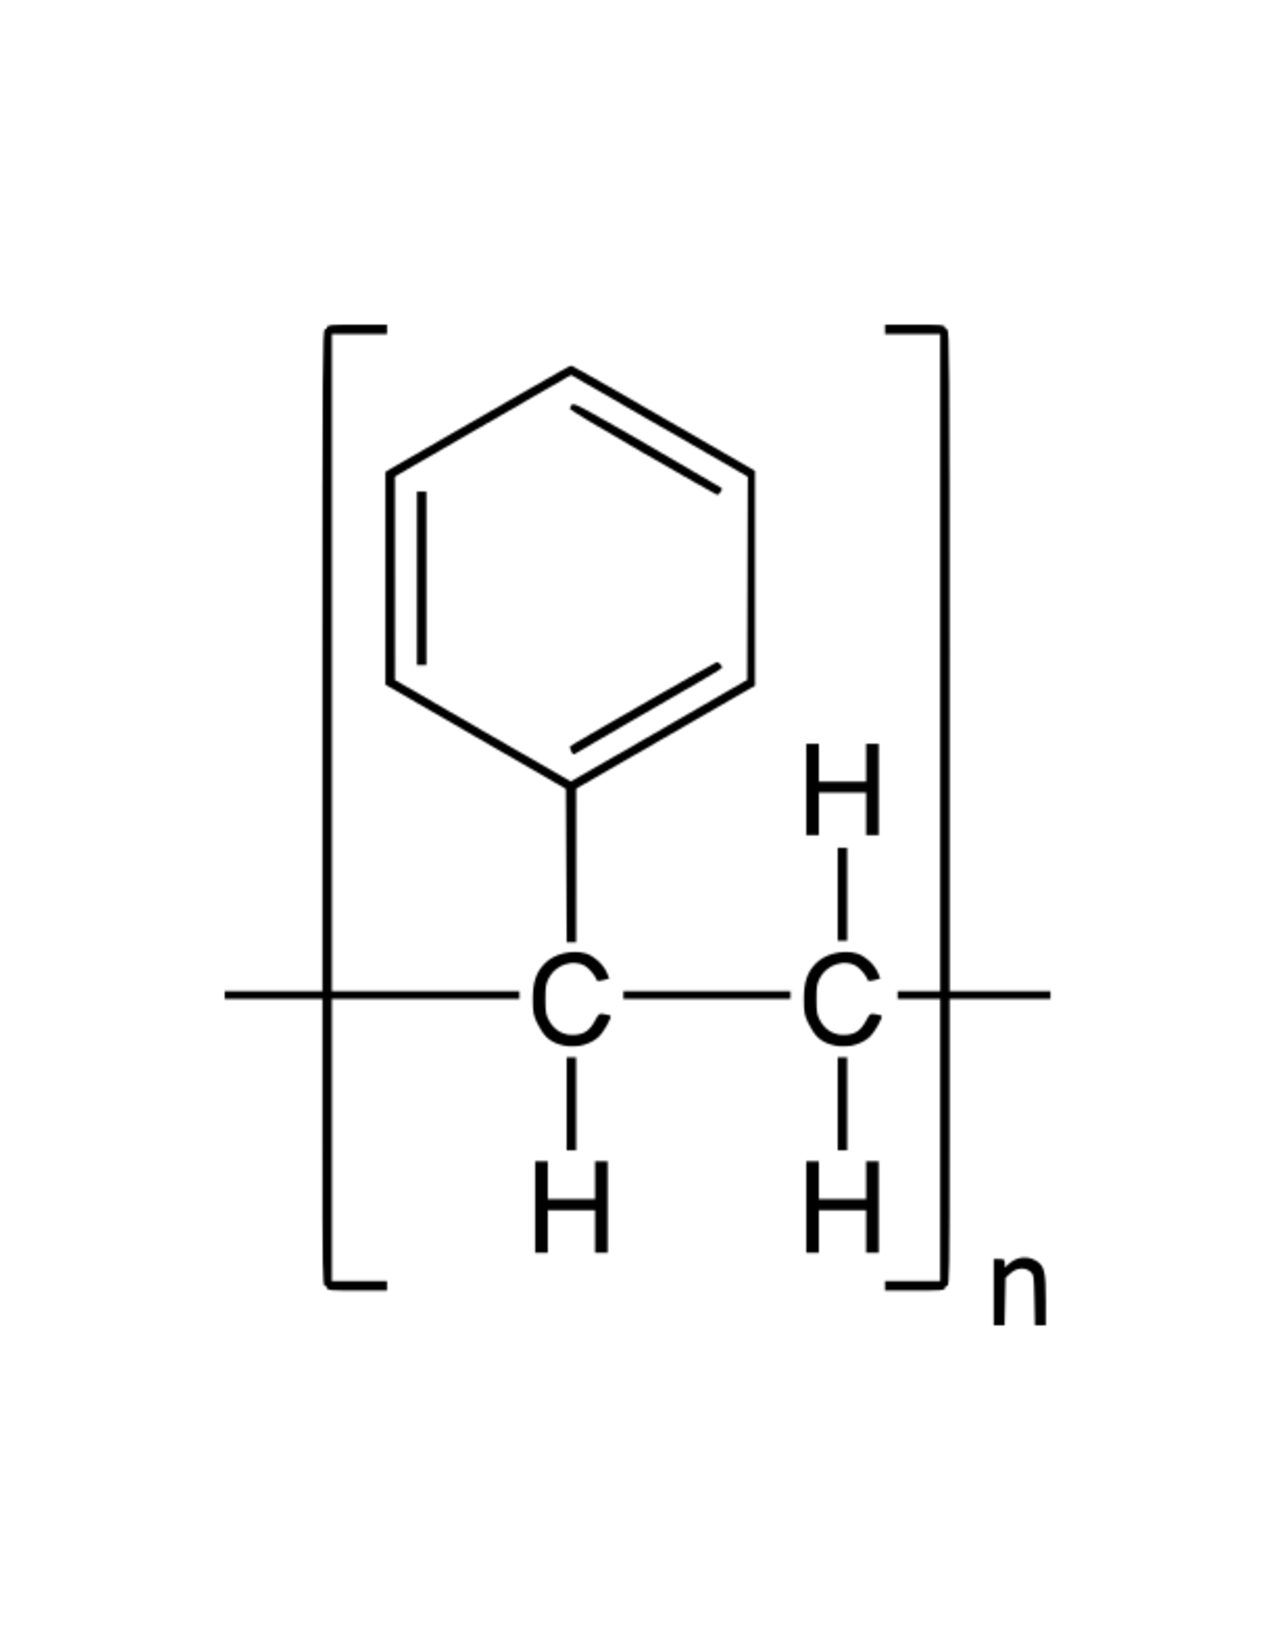
\includegraphics[width=6cm]{Polystyrene.pdf}}
      {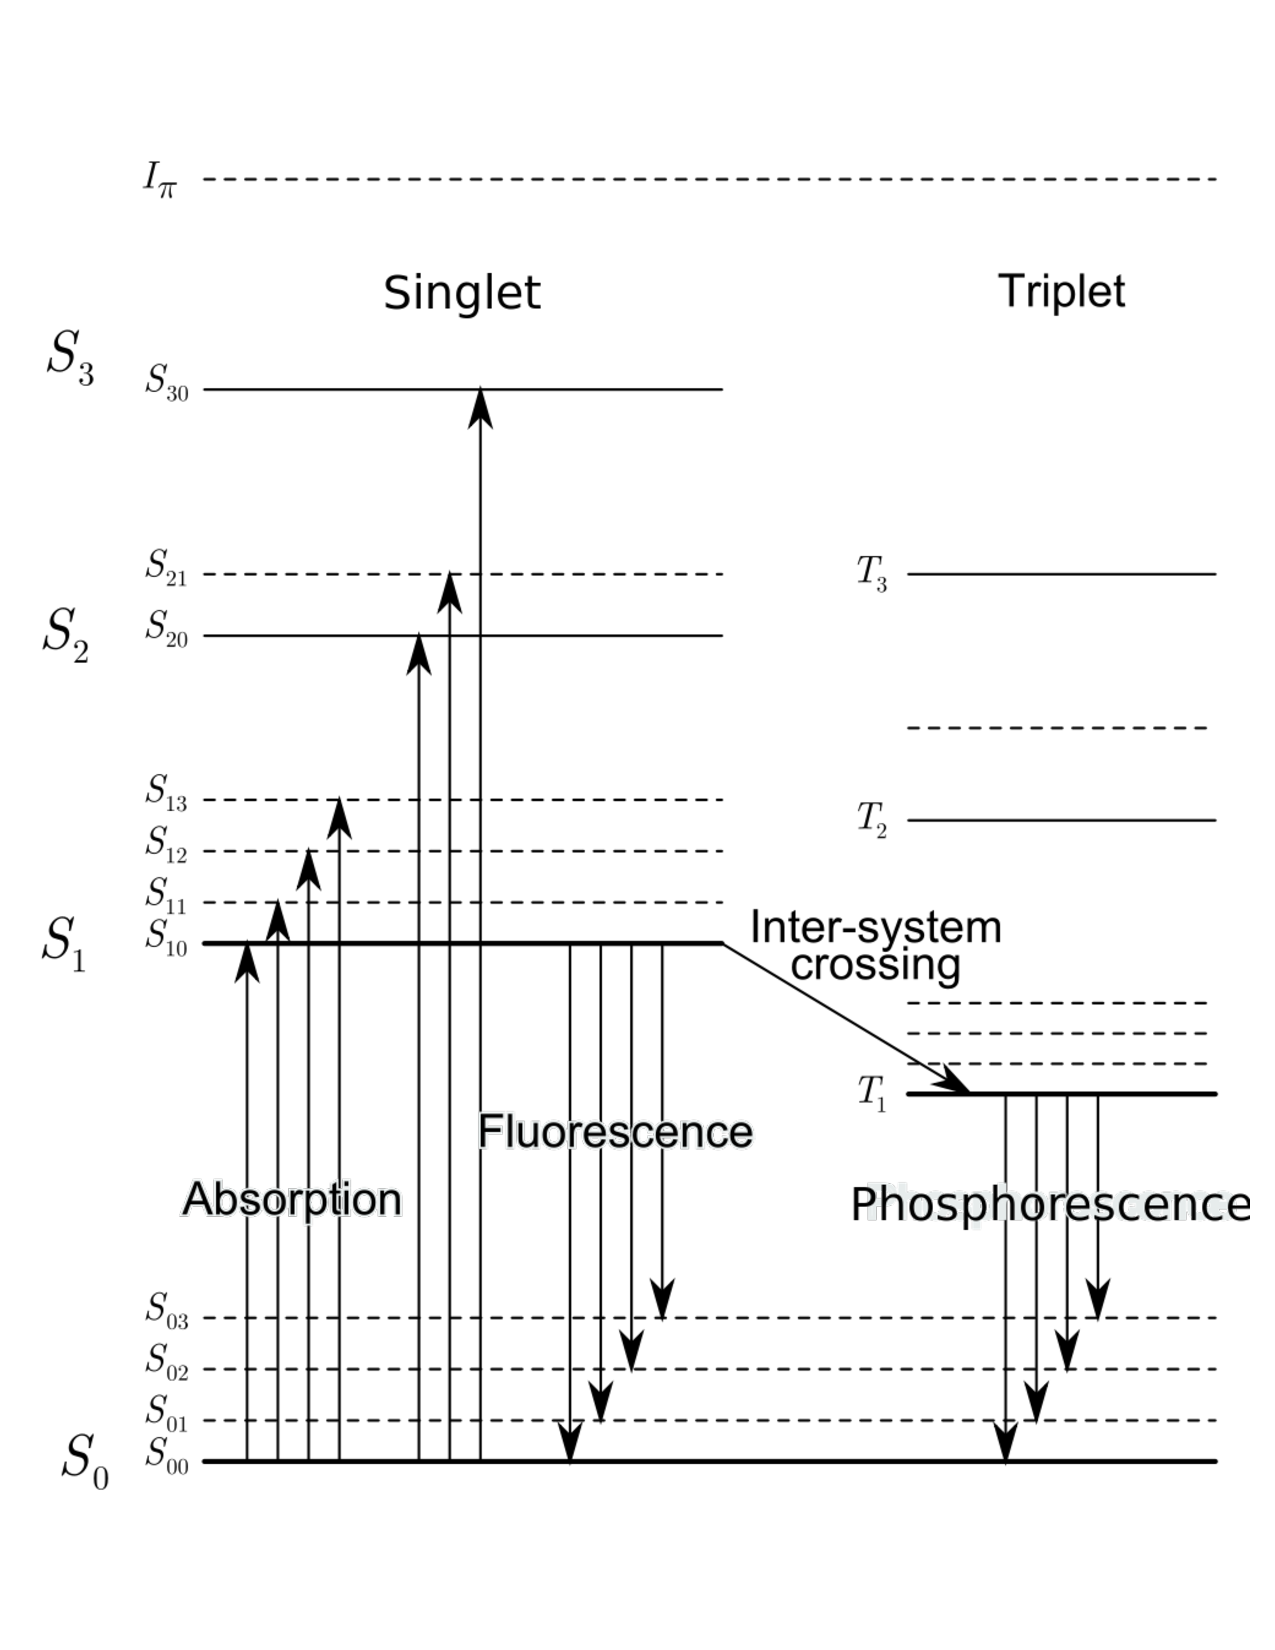
\includegraphics[width=6cm]{Pistates.pdf}}
\caption{
(a)
Basic chemical unit for polystyrene
(b)
typical energy levels in organic scintillators (stolen from Wikipedia)
}
\label{fig:polystyrene}
\end{figure}



In this type of scintillator, as described in \cite{birks}, 
a charged particle transversing the scintillator
excites the substrate.  The concentrations of the 
dopants are low enough that direct excitation is negligible.
In general, either the $\pi$ or $\sigma$ singlet electrons of the substrate
can be excited or ionized. 
Fast scintillation is generally related
to the excitation of the singlet $\pi$ electrons; the fraction
of the energy loss of the charged particle via this mechanism,
as opposed to the other possibilities such as excitation of
the triplet states or ionization, determines the scintillation
efficiency of the scintillator.  Typically, this probability is
two thirds of the fraction of electrons that are $\pi$ electrons \cite{birks}.
The excited singlet $\pi$ electrons can then either de-excite
through fluorescence (usually in the UV), 
non-radiative de-excitation (quenching, which can occur through internal collision, which is not affected by the molecule's environment
but is affected by its geometry which depends on the
polymer's history, and 
via inter-system crossing, which is strongly affected by 
the environment and the geometry/folding of the molecule,
as it needs magnetic perturbations to proceed \cite{brown}),
radiative migration of the excitation to another molecule
of the substrate, or non-radiative migration
to another molecule.  The radiative migration often involves UV light.
For crystals, exciton (the excited state)
diffusion  is the most important mechanism for
diffusion; for liquids, it is solvent-solvent resonance (transfer of the
excition via dipole-dipole interactions of two molecules)
and thermal diffusion (collisions)
\cite{birks}.
Migration is important for common scintillators, as this can transfer
the excitation of the substrate to the dopant, and 
thus lead to the emission
of the detectable light.  
The major mechanism that transfers the excitation from the substrate to the
primary dopant depends on the dopant concentration \cite{sauli}.  
At low concentrations, the primary mechanism is radiative.  As the
concentration increases, a non-radiative dipole-dipole exchanged
called ``Forster transfer''\cite{forster} becomes increasing important.  Both
of these processes depend on the spectral overlap between the
substrate and the primary dopant (the second even though it is non-
radiative).
A second dopant is often added to
shift the wave length of 
the light to one suitable for existing photo-detectors.
The primary transfer mechanism between the first and second 
dopant is radiative \cite{sauli}.
We refer to these two types of dopants 
as the primary dopant and the wavelength-shifting dopant.


\section{Radiation Damage in plastic scintillators}
Radiation damage
in scintillators was intensely studied during two periods:
during the late 1950's and early 1960's, when
scintillators were first being understood, and during the late 1980's
and early 1990's, when detectors for experiments at HERA, the SSC,
and the LHC were being designed.

Radiation damage was first observed by Birks and Black \cite{birksblack}
in pure anthracene crystals.
In \cite{rosmanzimmer}, from 1957, Rosman and Zimmer studied
 polystyrene and polystyrene with
different concentrations of paraterphenyl (PT) as primary dopant
and 1,1,4,4-tetraphenylbuadiene (TPB) as either a primary dopant or used
as a wave-length shifter for the PT.
They found that the radiation-induced self absorption
of light is stronger for shorter wavelengths.  They also found
that the number of induced color centers (which is the inverse 
of the absorption length) is linear in the dose.
Both results have been
confirmed by many studies for moderate doses ($<$ 5 Mrad),
at which point production of additional types of radicals opens up
and concentration saturation of the benzyle radical occurs,
resulting in an increase in the complexity of the damage \cite{harrah}.


While there were many studies of radiation damage by particle physicists
during the late 80's,
the most scholarly (meaning educational for
particle physicists who do not know much chemistry)
 are those of Klaus Wick and his diploma
students at the University of Hamburg 
\cite{34504},\cite{Wick1991472},\cite{289295},\cite{173180},\cite{467829},\cite{Wulkop1995141}
And by Bodman and Ulm, also from Hamburg \cite{Bodmann2001299},\cite{Bodmann2003495}.  Bross and Pla-Dalmau \cite{173178} also contains much useful
information, once you have learned enough chemistry to understand it.
Unfortunately, some of these works have
contradictory conclusions.
Most of these studies, however, concern the induced decrease
in absorption length, except for some very early studies
at very high doses and dose rates, and
an interesting discussion in
\cite{Wick1991472}, that we will discuss in detail later, on
decrease in light output.


In order to understand radiation damage to organic scintillators, it is important to
understand the basic chemistry involved.
In \cite{Wulkop1995141}, Wick {\it{et al.}} detail
the chemistry of radiation damage in polymers. 
When an ionizing particle interacts with the polymer substrate, it can
break the weak bonds the bind the oxygen, carbon, and hydrogen.
Todd\cite{todd} proposes that radiation first ruptures a C-H bond.
This can lead to the production
of radicals (such as  ${\rm \cdot CH_3}$,${\rm \cdot OCH_3}$,${\rm \cdot COOCH_3}$, where the $\cdot$ stands for a single dangling bond)
that absorb fluorescence light (color center) and lead to 
a permanent increase in light self absorption.
They can affect the environment of the other molecules, leading to
an increase of non-radiative decays.
When these bonds are broken, gas creation (evolution), polymer degradation (breakage 
of the polymer main chain (backbone) to the original monomer), 
and polymer cross linking
(when one or more polymer chains are joined by short, long, or even
polymeric molecules, usually by removal of a hydrogen,
although in polystyrene this also involves hydroperoxide groups due to removal of a water \cite{todd})
can also occur\cite{Wick1991472}.  
This again affects the local environment for the other molecules, and
can
change the energy levels for the broken strands, so that their
radiative transitions are no longer of appropriate wave length.
The change in energy levels can also enhance nonradiative decay modes.
For polystyrene, radical production and cross linking
are important \cite{Wick1991472}.  For other substrates, different
mechanisms can be dominant \cite{Wick1991472}.
According to the model described in ~\cite{kauffman}, polyene's
can form where a tertiary benzylic forms in the plastic under irradation.
The absorption of these bands depends on their length.  Longer bands
absorb at longer wave lengths, which may explain why the absorption bands
shift towards longer wave lengths after irradiation.
The result can be absorption of radiation,
less radiation and less transfer of the
excitation to the dopant.


Radicals
can migrate through the substrate, although the mechanisms for this
depend on whether or not oxygen is present.  If oxygen
is not present, migration occurs via hydrogen abstraction reactions.
However, when oxygen is present, additional reaction channels open.
Wick {\it{et al.}} list five additional migration mechanisms.
Note that cross linking of polymers severely reduces their
ability to migrate \cite{weir}.
Since radicals can
annihilate, migration can provide  a mechanism for
temporary light loss or temporary light self-absorption.   
Oxygen can change radicals
from types that absorb in the UV and visible to peroxide radicals,
which do not.  It is thought that this is the mechanism
through which ``bleaching'' of radiation damaged scintillator
occurs, after (or even during) the exposure (where bleaching
is a decrease in the radiation-induced self-absorption with time).
Note, however, that Oxygen is known be be a quenching molecule~\cite{sauli}, 
in that it absorbs photons responsible for the radiative transfer
from the substrate to the primary dopant.  For liquids, it is important
to avoid dissolved oxygen.

Since the effects depend in detail on the types and quantities
of the various different damage possibilities (the radicals produced,
the importance of cross-linking versus degradation, the mobility of
the molecules), the detailed result on the optical qualities
of the scintillator can vary.
For example, the behavior of scintillators
containing even small quantities of napthalene in the presence of oxygen is completely
different than those that do not, even when based
on the same substrate\cite{Wick1991472}.
Note also that some measurements \cite{todd} indicate
that discoloration (radiation-induced absorption length) 
of polystyrene in vacuum is only due
to radical production from manufacturing impurities, perhaps
interacting with oxygen, and not due to radical production
from the polystyrene itself.
The manufacturing method for the substrate
and temperature treatment during manufacturing
can have a strong effect \cite{bicken} \cite{johnson},
as this can effect polymerization, content of gases, the
diffusion constant, and mobility of radicals.  Heating
of the plastic after irradiation is another way, beyond
oxygen diffusion, to increase
the mobility of the radicals and remove color centers.
Polystyrene is especially sensitive to temperature treatment
\cite{bicken}.  If exposed to temperatures above ${\rm 70^o}$C
before or after irradiation, the damage is increased.

Wick {\it{et al.}} \cite{Wick1991472}
have done many studies on the influence of the diffusion of oxygen on
induced self absorption
in materials like polystyrene and PMMA
(polymethyl methacrylate).  
They show that the penetration depth of oxygen into the substrate
depends on the dose rate, presumably because interactions
of the oxygen with radicals affects its ability to diffuse.  
At lower dose rates, oxygen penetrates
more deeply.  Because of the importance of the interaction
of oxygen with radicals, this can lead to dose rate effects
for radiation damage.  They also show that the recovery of the
induced self absorption after irradiation (bleaching)
is consistent with
oxygen diffusion.  They show that there is little bleaching
without oxygen, and that a very large number of color centers
form if there is no oxygen, although the permanent damage after
bleaching (exposure to oxygen after the radiation) is slightly
larger if there is oxygen.
A similar discussion exists in Bross and Pla-Dalmau \cite{173178}.
They looked at dose rates of 1 Mrad/h and 0.03 Mrad/h for a
total dose of 10 Mrad.  They found no dose rate effect in
inert atmospheres, confirming the role of oxygen for permanent
induced absorption.  They found more permanent damage if the samples
were in a pressurized oxygen atmosphere (2 atm.), although
they also comment that annealing (reduction of the non-permanent losses)
is aided by oxygen.
In general, oxygen during irradiation seems to increase the permanent
damage, even after annealing.  However, if there is no oxygen present,
there is no annealing, and the induced self absorption can be very large.
In \cite{Wulkop1995141}, Wick develops a model that explains
both the temporary light self absorption
and its time dependence, and permanent induced self-absorption in
terms of oxygen diffusion.
An interesting study of dose rate effects on the absorption length
in plastic fibers is in \cite{zorn2}.  
He finds that permenant damage in the presense of oxygen depends
on both the dose rate and the atmosphere.  At low dose rates,
an inert atmosphere is better but at high dose rates, one containing 
oxygen is better.
Also, in \cite{zorn3}, results on a replacement substrate
that may be more radiation resistant than PVT or PS are presented.
In general, polyvinylxylene is more radiation resistant than PVT, which
is better than PS \cite{sauli}.

Studies on the effect of radiation on the light yield are fewer
than those on self-absorption.
In an early study, Rosman and Zimmer found, after correcting
for any induced self-absorption, that the light
output versus dose is described,
approximately and for relatively large dose rates, by a double exponential, 
with a small-dose component whose constant is approximately 100 Mrad,
a large dose even by modern standards.
The exponential constant was smallest for pure polystyrene, while
that of polystyrene doped with 1.5\% PT  and 0.02\%TPB
was slightly larger.  The constant was considerably larger (less
self-absorption of light) for 3\% TPB.  They also used UV light to illuminate
the samples with 1.5\% TPB, and found that this showed less
reduction of light than excitation via charged particles.
Since the polystyrene substrate is transparent to UV, this
indicates that the TPB was not damaged, and instead the damage
should be either to the polystyrene or the migration of the polystyrene
to the dopant.

In \cite{berlman}, from 1958, Berlman studied liquid scintillators
that used xylene as the substrate and diphenyloxazole (PPO) as the dopant.
He found that the decrease in light output with dose could be
reduced with higher concentrations of dopant.  He also found
that if irradiated dopant is put into an unirradiated substrate,
the light output is still good.  His studies
confirm that
an important source of the reduction of light output is due to
reduced migration from the substrate 
to the dopant or deexcitation of the substrate via heat.
A 1992 study by Bross and Pla-Dalmau, using polystyrene,
reached similar conclusions \cite{173178}.

In another study by Bross, Pla-Dalmau \it{et al.} from 1991, the authors look at light output for various primary and seconary dopants for a dose of 10 Mrad accumulated with a relatively high (0.4 Mrad/h) dose rate.  They looked at this for 2 different concentrations of the secondary dopant.  They optimized the concentration of the first dopant using the light output before irradation.  They found no change to the intrinsic light output, indicating at high dose rates the dopants were
not damaged by this large dose.  


In \cite{Wick1991472}, Wick also studies decreased light
output for a plastic scintillator from Kuraray, SCSN-38, which
is based on polystyrene with b-PBD and BDB dopants.
The main absorption wavelengths for polystyrene typically range between
between 230 to 260 nm, for the primary dopant b-PBD between 270 to 330 nm,
and for the wavelength shifting dopant BDB between 310 to 400 nm.
They found that light loss was much stronger in the presence of oxygen.
Note that while oxygen plays a beneficial role in regards
to annealing of induced absorption length at the end of radiation, 
it plays a detrimental role in 
regards to light output.  
They also found the light output loss
was independent of the wavelength of the light
that was used to excite the scintillator, when it
was varied between 230 and 400 nm.
From this they conclude that the damage is due to destruction
of the second flour.  This is different than what was found in
earlier studies, which indicated that damage to the dopants was
small and that damage was mostly to the substrate,
although different dopants were used.
By looking at the damage as a function of the thickness of the scintillator,
they concluded that the BDB molecules are mainly destroyed
near the surface, which lends support to a mechanism involving
oxygen diffusion.

If the damage is due to oxygen diffusion, a dose rate effect
is expected.
An interesting new result is due to Biagtan {\it{et al.}} \cite{Biagtan1996125}, in 1996.  They look at light output reduction for two
polystyrene-based scintillators (SCSN-38 and SCSN-81) and a
polyvinyltoluene-based scintillator (Bicron-499-35).  
They find a reduction in light output that depends linearly on the
log of the dose rate for dose rates ranging from $0.01$ to
$2$ Mrad/hr.  Note that the effect is not small: for a
dose of 2 Mrad, the light loss is negligible for a dose rate
of 2 Mrad/hr but 20\% for a dose rate of 0.01 Mrad/hr for SCSN-81.

If this dose rate effect is due to oxygen diffusion, then
we expect it to be governed by the diffusion equation.  Since
the oxygen diffusion depth is greater at lower dose rates,
we expect the damage for the same dose at different dose rates to
increase up to the point where the dose rate is low enough that oxygen
permeates the entire sample.  The dose rate effect should plateau
at this point.  Specifically, we predict that the light output
reduction should depend on both the dose and the dose rate as:
$$ L(R,D) = 1 - [f(D)Z(R) + a(D)(1-Z(R))]$$
where L is the \% light yield, D is the dose, R is the dose rate, 
Z(R) is the fraction of the scintillator containing 
oxygen and is given by $min({{2 z_0(R)}\over{d}},1)$
where d is the thickness of the scintillator and $z_0$ gives
the depth of scintillator penetrated by oxygen,
a(D) is related to the fraction of quenching in the part of
the scintillator containing oxygen and is given by $1-e^{-a_0 D}$, 
and
f(D) is related to the fraction of quenching in the part of
the scintillator not containing oxygen and is given by $1-e^{-f_0 D}$.
The diffusion depth $z_0(R)$ is given by diffusion theory as 
$$z_0(R)=\sqrt{\gamma/R}$$
where $\gamma$ is a property of the substrate and the radicals that
are dissolved in that substrate during the diffusion process.
The value for $\gamma$ depends on the material, oxygen pressure,
radical concentration (which is proportional to the dose) and 
temperature.
The minimization in Z(R) occurs because the fraction of scintillator
containing oxygen can not exceed one.  Note that this equation 
assumes the temperature and the surrounding atmosphere
is held constant, as this can 
affect diffusion.

Figure \ref{fig:kevinfit} shows a fit of our theory to the Biagtan data 
\cite{Biagtan1996125} for SCSN-81 and for B-499-35.  The fit is not bad,
with 
$\gamma$ of 0.35 $\pm$ 0.007, $f_0$ of 0.092 $\pm$ 0.005,
and $a_0$ of 0.029 $\pm$ 0.003 
for SCSN-81.  For B-499-35, the results
are 
$\gamma$ of 0.092 $\pm$ 0.012, $f_0$ of 0.088 $\pm$ 0.004,
and $a_0$ of 0.006 $\pm$ 0.003. 
The model clearly predicts a knee when the rate $R={{4 \gamma}\over{d^2}}$.
For the Biagtan data, this is at a dose rate of $10^{-2}$ Mrad/hr, which is
slow for a reactor test but large for actual operating detectors.
The data, unfortunately, does not extend below dose rate of this value,
except for the very largest doses.  As explained in \cite{harrah},
the chemistry of radiation damage changes for doses
around 5 Mrad.
The model also predicts that the knee should occur at higher
dose rates for thinner scintillator, but no data is available
on this either.


Logically, also,
the linear trend seen  in the log of the dose rate must fail at 
very low dose rates, and some kind of knee must eventually occur.  
Unfortunately, real detectors operate at these very low dose rates,
and there is no data or verified model to do the extrapolation.



\begin{figure}[!htbp]
\centering
    {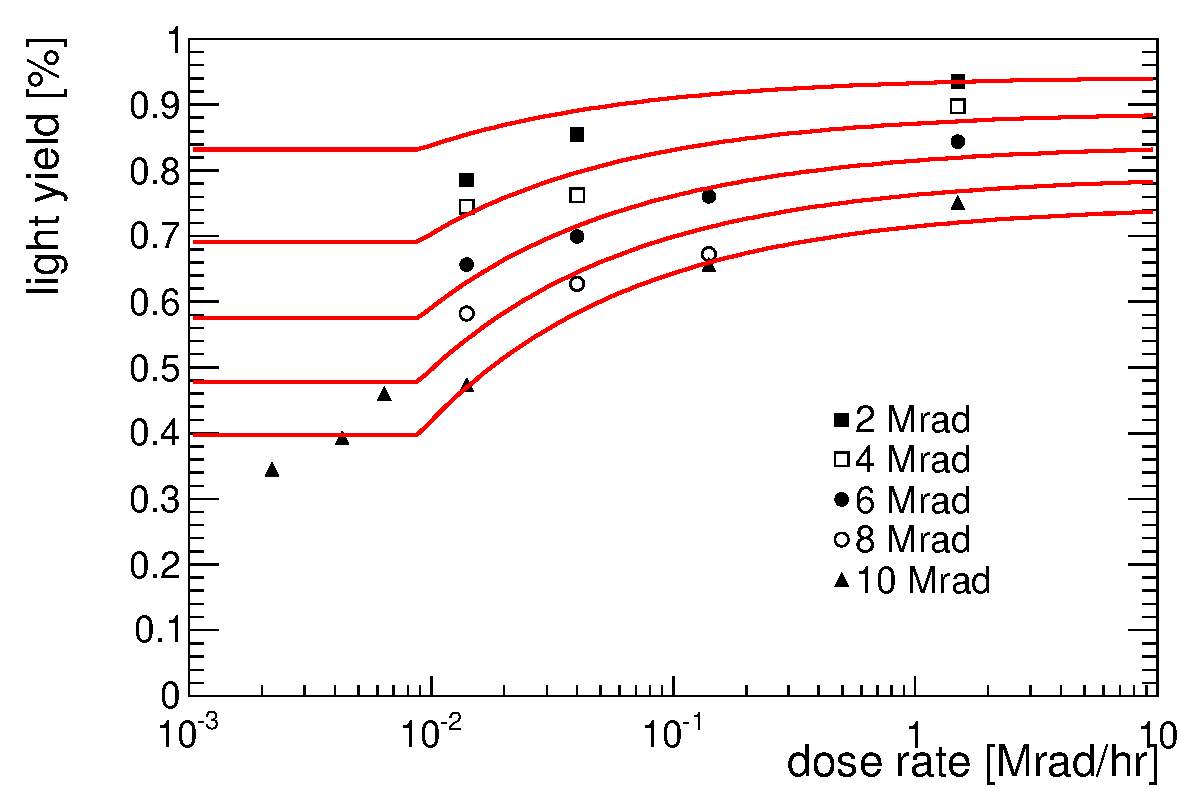
\includegraphics[width=6cm]{fitWick8s.pdf}}
    {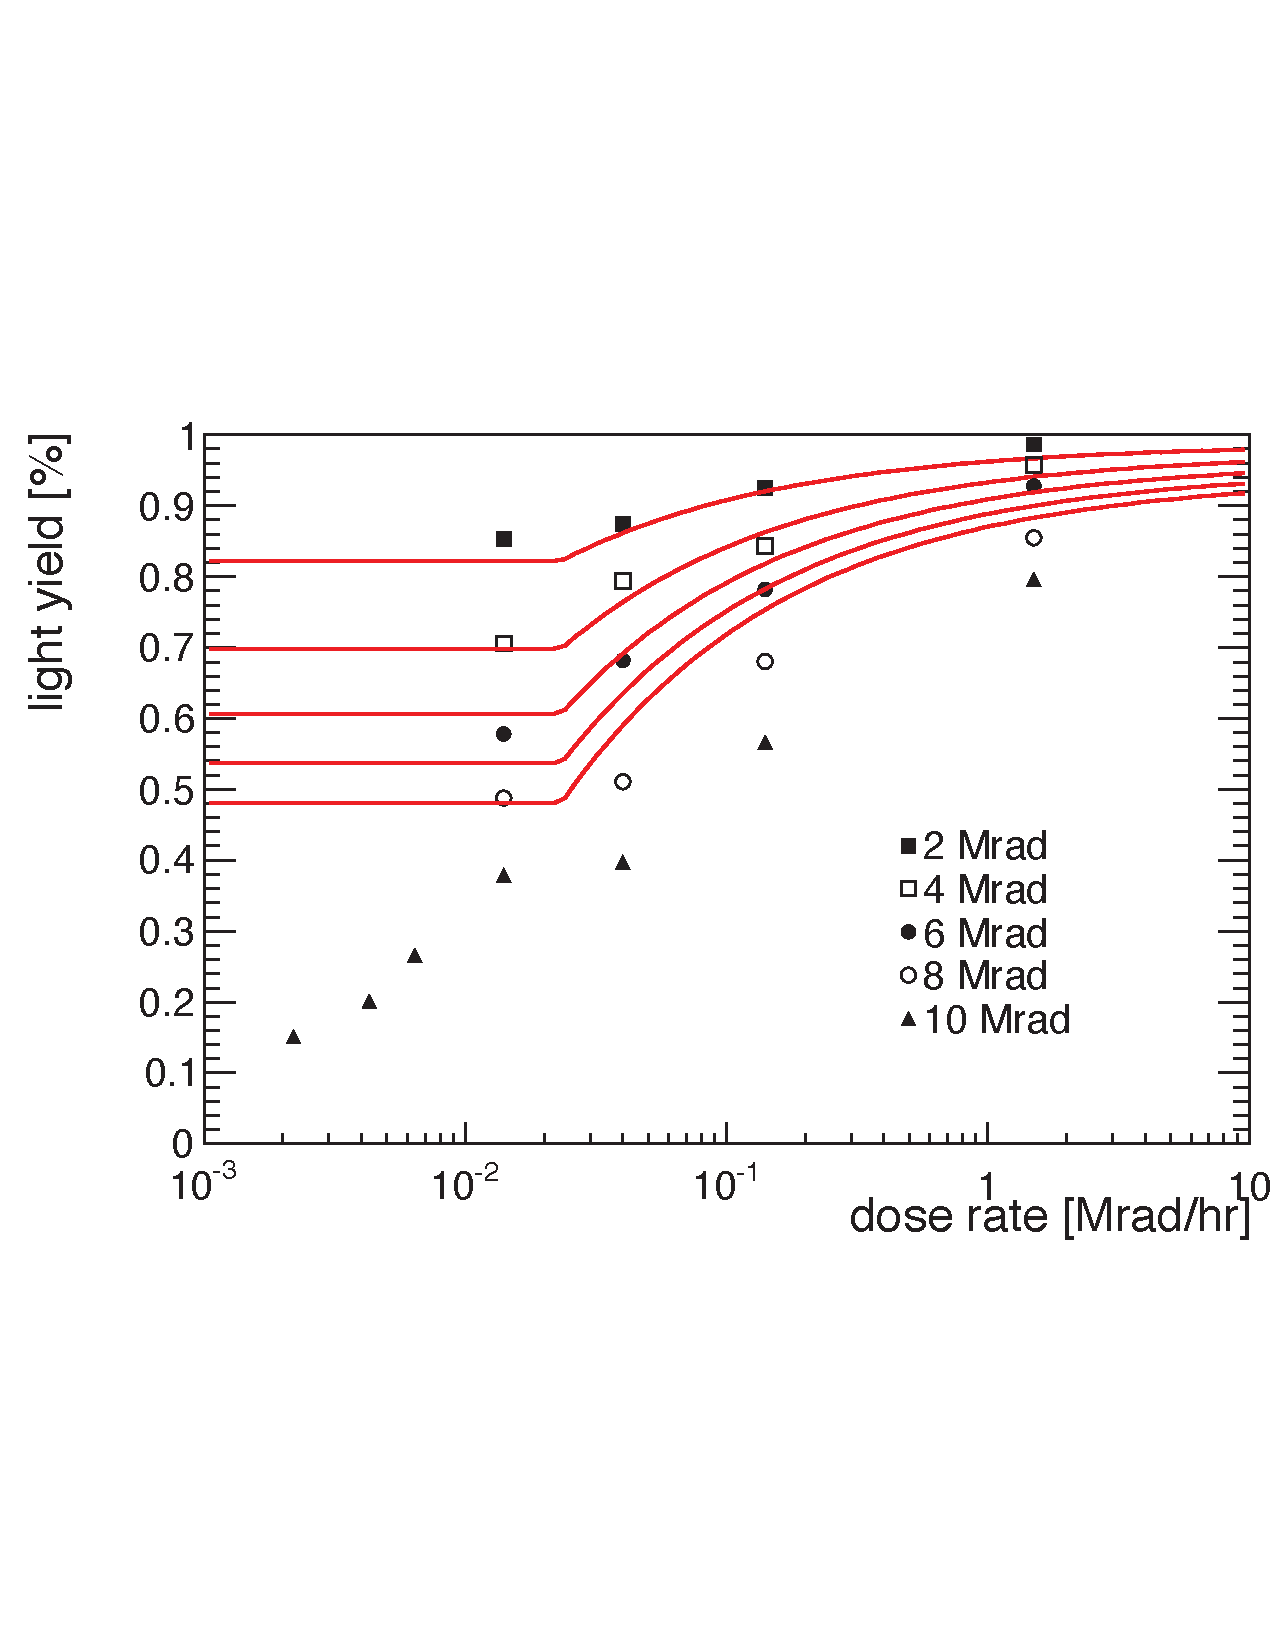
\includegraphics[width=6cm]{fitWick10bll.pdf}}
\caption{
Fit of our model for the fractional light output relative to
unirradiated scintillator as a function of both total dose
and the dose rate
to the Biagtan data \cite{Biagtan1996125}
for SCSN-81, which uses polystyrene as its substrate (top) and 
B-499-35, which uses polyvinyltoluene (bottom).
}
\label{fig:kevinfit}
\end{figure}

While there are still mysteries on solid plastic scintillators
fluorescing in the blue, very little
published data is available on liquid scintillators and
on scintillators operating at longer wave lengths than blue.
A 1992 paper by Bross and Pla-Dalmau \cite{173178} shows that using
a 3HF dopant does that scintillators operating at longer
wave lengths are less affected by radiation damage.  
There is no information on dose-rate effects.  
The published works on liquid scintillators that we were able
to find was by Zorn \cite{zornliquid} in 1990, the paper
discussed previously from Berlman in 1958, and a paper
by Klein from 1967\cite{Klein1967399}.  
There are papers on using scintilators in capilaries for calorimetry\cite{white}.
There is also
unpublished work from CDF using Bicron517L\cite{kenichi1} and
\cite{kenichi2}.
There is also an unreferred difficult-to-obtain conference
proceeding on pyrex tubes filled with liquids \cite{fsuliquid}.
Neither measure
the properties of modern liquid scintillators that are rumored
to be radiation resistant.


